\documentclass[12pt,a4paper]{article}

% ── packages ────────────────────────────────────────────────────────────────
\usepackage[a4paper, top=2.5cm, bottom=2.5cm, left=3cm, right=2.5cm]{geometry}
\usepackage{amsmath, amssymb, amsthm}
\usepackage{graphicx}
\usepackage{booktabs, array, longtable}
\usepackage{listings, xcolor}
\usepackage{hyperref}
\usepackage{parskip}
\usepackage{setspace}
\usepackage{fancyhdr}
\usepackage{titlesec}
\usepackage{mdframed}
\usepackage{enumitem}
\usepackage{tikz}
\usetikzlibrary{shapes.geometric, arrows.meta, positioning, fit, backgrounds}
\usepackage{caption}
\usepackage{float}
\usepackage{microtype}
\usepackage{soul}   % for \hl highlights

\onehalfspacing

% ── colours ─────────────────────────────────────────────────────────────────
\definecolor{codebg}{HTML}{F8F8F8}
\definecolor{boxbg}{HTML}{EBF5FB}
\definecolor{boxline}{HTML}{2471A3}
\definecolor{failbg}{HTML}{FDEDEC}
\definecolor{failline}{HTML}{C0392B}
\definecolor{successbg}{HTML}{EAFAF1}
\definecolor{successline}{HTML}{1E8449}
\definecolor{kwcol}{HTML}{0000BB}
\definecolor{cmtcol}{HTML}{228B22}
\definecolor{strcol}{HTML}{BB0000}

% ── code style ──────────────────────────────────────────────────────────────
\lstdefinestyle{mypy}{language=Python,
  backgroundcolor=\color{codebg}, frame=single,
  rulecolor=\color{gray!40}, basicstyle=\small\ttfamily,
  keywordstyle=\color{kwcol}\bfseries,
  commentstyle=\color{cmtcol}\itshape,
  stringstyle=\color{strcol},
  numbers=left, numberstyle=\tiny\color{gray},
  numbersep=7pt, breaklines=true,
  showstringspaces=false, tabsize=4, captionpos=b}
\lstset{style=mypy}

% ── insight / failure / success boxes ───────────────────────────────────────
\newmdenv[backgroundcolor=boxbg, linecolor=boxline, linewidth=2pt,
  leftline=true, rightline=false, topline=false, bottomline=false,
  innerleftmargin=10pt, innerrightmargin=6pt,
  skipabove=8pt, skipbelow=6pt]{insight}

\newmdenv[backgroundcolor=failbg, linecolor=failline, linewidth=2pt,
  leftline=true, rightline=false, topline=false, bottomline=false,
  innerleftmargin=10pt, innerrightmargin=6pt,
  skipabove=8pt, skipbelow=6pt]{failbox}

\newmdenv[backgroundcolor=successbg, linecolor=successline, linewidth=2pt,
  leftline=true, rightline=false, topline=false, bottomline=false,
  innerleftmargin=10pt, innerrightmargin=6pt,
  skipabove=8pt, skipbelow=6pt]{successbox}

% ── theorem envs ────────────────────────────────────────────────────────────
\newtheorem{theorem}{Theorem}
\newtheorem{lemma}[theorem]{Lemma}
\newtheorem{corollary}[theorem]{Corollary}
\newtheorem*{remark}{Remark}

% ── shortcuts ───────────────────────────────────────────────────────────────
\newcommand{\R}{\mathbb{R}}
\newcommand{\norm}[1]{\left\lVert#1\right\rVert}
\newcommand{\diag}{\operatorname{diag}}

% ── header ──────────────────────────────────────────────────────────────────
\pagestyle{fancy}\fancyhf{}
\fancyhead[L]{\small Risk-Aware Hybrid LQR-MPC Navigation}
\fancyhead[R]{\small\thepage}
\renewcommand{\headrulewidth}{0.4pt}

\hypersetup{colorlinks=true, linkcolor=blue!70!black,
  citecolor=teal, urlcolor=blue!80!black}

% ── section style ────────────────────────────────────────────────────────────
\titleformat{\section}{\large\bfseries}{}{0em}{}[\titlerule]
\titleformat{\subsection}{\normalsize\bfseries}{}{0em}{\textbullet\ }

%% ═══════════════════════════════════════════════════════════════════════════
\begin{document}

% ── Title ────────────────────────────────────────────────────────────────────
\begin{titlepage}
\centering
\vspace*{3cm}
{\LARGE\bfseries Risk-Aware Hybrid LQR-MPC Navigation\\[0.4em]
for Autonomous Systems\par}
\vspace{0.6cm}
{\large\itshape Project Report — From Idea to Hybrid Controller\par}
\vspace{2cm}
\begin{tabular}{ll}
  \textbf{Author:}      & Erebuzzz \\[4pt]
  \textbf{Repository:}  & \small\url{https://github.com/Erebuzzz/Risk-Aware-Hybrid-LQR-MPC-}\\
                        & \small\url{Navigation-for-Autonomous-Systems} \\[4pt]
  \textbf{Date:}        & March 2026 \\[4pt]
  \textbf{Status:}      & In Progress (up to Hybrid Controller)
\end{tabular}
\vspace{2cm}

\noindent\rule{0.85\linewidth}{0.5pt}
\vspace{0.4cm}

\begin{minipage}{0.85\linewidth}
\textbf{Abstract.}
This report documents the design and development of an autonomous navigation
system for a differential-drive robot. Rather than a polished summary of
results, this is a record of the whole process: what we tried, what broke,
why we changed direction, and where we ended up. The system went through
three major phases --- a baseline LQR tracker, adding obstacle avoidance
with MPC, and finally combining the two into a smooth hybrid controller.
At each stage we hit real engineering problems and had to rethink our
approach. The final hybrid controller blends LQR and MPC continuously
rather than switching between them, which turned out to produce significantly
smoother control signals and better tracking accuracy.
\end{minipage}

\noindent\rule{0.85\linewidth}{0.5pt}
\end{titlepage}

\tableofcontents
\clearpage

%% ─────────────────────────────────────────────────────────────────────────
\section{Where We Started: The Problem}
%% ─────────────────────────────────────────────────────────────────────────

We wanted to build a navigation system for a differential-drive robot that
could follow a reference trajectory while avoiding obstacles in its path.
Sounds straightforward, but it turned out to be a lot more involved than
expected.

The core tension we noticed right away: trajectory tracking and obstacle
avoidance want very different things from the controller. A good trajectory
tracker stays smooth and energy-efficient --- it doesn't want to be
disturbed unless it has to. Obstacle avoidance, on the other hand, needs to
be reactive and sometimes aggressive. If you design for one, you compromise
the other.

The robot model we used is the standard unicycle (differential drive):
\begin{equation}
  \dot{x} = v\cos\theta, \quad \dot{y} = v\sin\theta, \quad \dot{\theta} = \omega
\end{equation}
where the state is position and heading $\mathbf{x} = [x, y, \theta]^\top$
and the inputs are linear velocity $v$ and angular velocity $\omega$. We
constrained these to $|v| \leq 2.0\,\text{m/s}$ and
$|\omega| \leq 3.0\,\text{rad/s}$ to stay physically reasonable. The
simulation runs at 50\,Hz (timestep $dt = 0.02\,\text{s}$).

For a reference trajectory we used a Lissajous figure-8:
\[
  x_r(t) = 2\sin(t), \quad y_r(t) = 2\sin(0.5t)
\]
This was a good test case because it forces the robot through curved turns
(where obstacle encounters are likely) and straight sections (where smooth
tracking matters most).

%% ─────────────────────────────────────────────────────────────────────────
\section{Development Timeline}
%% ─────────────────────────────────────────────────────────────────────────

Before diving into the technical details, here is a rough timeline of how
the project evolved. Each phase taught us something that fed into the next.

\begin{figure}[H]
\centering
\begin{tikzpicture}[
  node distance=0pt,
  box/.style={draw, rounded corners=4pt, text width=3.2cm,
    minimum height=1.1cm, align=center, font=\small},
  okbox/.style={box, fill=successbg, draw=successline!70!black},
  failbox2/.style={box, fill=failbg, draw=failline!70!black},
  arrow/.style={-{Stealth[length=8pt]}, thick, color=gray!60},
  note/.style={font=\footnotesize\itshape, text=gray},
]
% Row 1 — main flow
\node[okbox] (lqr) {Phase 1\\LQR Baseline\\{\tiny Tracking only}};
\node[okbox, right=1.2cm of lqr] (mpc) {Phase 2\\MPC + Obstacles\\{\tiny CVXPY/OSQP}};
\node[failbox2, right=1.2cm of mpc] (hs) {Phase 3\\Hard Switch\\{\tiny Jerk problem}};
\node[okbox, right=1.2cm of hs] (hyb) {Phase 4\\Smooth Hybrid\\{\tiny Where we are}};

\draw[arrow] (lqr) -- (mpc);
\draw[arrow] (mpc) -- (hs);
\draw[arrow] (hs) -- (hyb);

% Failure annotations below
\node[note, below=0.55cm of mpc, text width=3.2cm, align=center]
  (mpcnote) {Latency: 180ms\\DCP errors\\Too slow};
\node[note, below=0.55cm of hs, text width=3.2cm, align=center]
  (hsnote) {Jerk spikes at\\transitions,\\Zeno chattering};

\draw[-{Stealth[length=5pt]}, dashed, gray!50] (mpcnote.north) -- (mpc.south);
\draw[-{Stealth[length=5pt]}, dashed, gray!50] (hsnote.north) -- (hs.south);

% Sub-milestones below Phase 2
\node[failbox2, below=1.8cm of lqr, text width=3.0cm, minimum height=0.9cm,
  font=\footnotesize, align=center]
  (dcperr) {DCP Error:\\circular constraints\\rejected by CVXPY};
\node[okbox, right=0.6cm of dcperr, text width=3.0cm, minimum height=0.9cm,
  font=\footnotesize, align=center]
  (halfplane) {Fixed with\\half-plane\\linearisation};
\draw[arrow] (dcperr) -- (halfplane);

% CVXPYgen fail
\node[failbox2, below=0.5cm of dcperr, text width=3.0cm, minimum height=0.9cm,
  font=\footnotesize, align=center]
  (cvxfail) {CVXPYgen install\\failed (Windows +\\Python 3.13)};
\node[okbox, right=0.6cm of cvxfail, text width=3.0cm, minimum height=0.9cm,
  font=\footnotesize, align=center]
  (paramfix) {Fixed with CVXPY\\Parametrisation\\(38× speedup)};
\draw[arrow] (cvxfail) -- (paramfix);

\end{tikzpicture}
\caption{Project development path. Red boxes mark things that failed;
  green boxes mark working outcomes.}
\label{fig:timeline}
\end{figure}

The rest of this report follows the same order: we start with Phase 1 and
walk through each decision and failure until we reach the current hybrid
controller design.

%% ─────────────────────────────────────────────────────────────────────────
\section{Phase 1 --- LQR: Getting the Robot to Follow a Path}
%% ─────────────────────────────────────────────────────────────────────────

The first thing we built was a simple LQR controller. The idea is
straightforward: given a reference trajectory, define the error
$\mathbf{e}_k = \mathbf{x}_k - \mathbf{x}^r_k$ and find the gain matrix
$K$ that drives this error to zero in the most energy-efficient way.

Formally, the LQR minimises:
\[
  J = \sum_{k=0}^{\infty} \left( \mathbf{e}_k^\top Q_{\text{lqr}}\,
  \mathbf{e}_k + \mathbf{u}_k^\top R_{\text{lqr}}\, \mathbf{u}_k \right)
\]
The matrices $Q_{\text{lqr}} = \diag(15, 15, 8)$ and
$R_{\text{lqr}} = \diag(0.1, 0.1)$ were tuned manually --- the heading
weight was lower than position because heading error naturally self-corrects
as the robot moves. Solving the Discrete Algebraic Riccati Equation (DARE)
gives the optimal gain:
\[
  K = (R_{\text{lqr}} + B^\top P_\infty B)^{-1} B^\top P_\infty A, \qquad
  \mathbf{u}_k^{\text{LQR}} = -K\,\mathbf{e}_k.
\]

\subsection{The heading wrap problem}

The one thing that caught us out here was heading angle wrapping. The error
$\theta - \theta_r$ can jump from $+\pi$ to $-\pi$ if the reference crosses
the $\pm\pi$ boundary. Without wrapping it to $(-\pi, \pi]$, the LQR
controller would try to rotate the robot the long way around and spiral
out of control. Once we added the wrap, the controller became stable.

\begin{insight}
\textbf{Takeaway from Phase 1.} LQR works well on open tracks. In 20
obstacle-free test runs, it maintained tracking error below 0.5\,m
throughout. The gain computation takes microseconds. But it has no
concept of obstacles --- it would drive straight through walls without
hesitation.
\end{insight}

%% ─────────────────────────────────────────────────────────────────────────
\section{Phase 2 --- MPC: Adding Obstacle Avoidance}
%% ─────────────────────────────────────────────────────────────────────────

Once the LQR was working, we needed obstacle avoidance. The standard tool
for this is Model Predictive Control (MPC), which online-solves a short
optimization over a future horizon $N$ at each control step. The key
advantage: you can directly encode ``don't hit obstacle $i$'' as a
constraint in the optimization.

The basic MPC problem we formulated:
\begin{align}
  \min_{\mathbf{u}_{0:N-1}} \quad &
    \sum_{k=0}^{N-1} \left( \norm{\mathbf{x}_k - \mathbf{x}^r_k}_Q^2
    + \norm{\mathbf{u}_k}_R^2 \right)
    + \norm{\mathbf{x}_N - \mathbf{x}^r_N}_P^2 \\
  \text{s.t.} \quad &
    \mathbf{x}_{k+1} = A_d \mathbf{x}_k + B_d \mathbf{u}_k \\
  & |v_k| \leq 2.0, \quad |\omega_k| \leq 3.0 \\
  & \text{obstacle avoidance (see below)}
\end{align}
We used a horizon of $N = 5$ steps ($0.1\,\text{s}$ lookahead) and solved
it with CVXPY backed by OSQP. The linearised dynamics matrices $A_d, B_d$
were recomputed at each step around the current reference point --- making
this a Linear Time-Varying MPC.

\subsection{Failure: Circular obstacle constraints rejected by CVXPY}

The natural way to keep the robot away from a circular obstacle centred at
$c_i$ with radius $r_i$ is:
\[
  \norm{[x_k, y_k]^\top - c_i}^2 \geq (r_i + d_{\text{safe}})^2
\]

We added this and ran the code. CVXPY crashed immediately:

\begin{failbox}
\textbf{Error encountered:}
\begin{verbatim}
DCPError: Problem is not DCP.
Expression norm(x - c, 2)**2 is not DCP.
\end{verbatim}
The squared norm on the left side of $\geq$ is convex, and CVXPY's DCP
rules require the left side of $\geq$ to be concave. So this formulation
was invalid. We spent some time reading CVXPY documentation before
understanding why.
\end{failbox}

\textbf{The fix.} We replaced the exact circular constraint with a linear
half-plane approximation. Around the current robot position, the nearest
point on the obstacle boundary defines an outward normal $\hat{n}_i$. The
linearised constraint is:
\[
  \hat{n}_i^\top [x_k, y_k]^\top \geq r_i + d_{\text{safe}} - \xi_i,
  \qquad \xi_i \geq 0
\]
The slack variable $\xi_i$ with a penalty $\rho \xi_i^2$ (we used
$\rho = 5000$) prevents the QP from becoming infeasible in tight spaces.
This is a standard technique, and it worked fine. The linearisation
approximation is only tight near the current position, but for $N=5$
steps it is accurate enough.

\subsection{Failure: The solver was way too slow}

The MPC produced correct obstacle-avoiding trajectories. But it was unusably
slow. Each solve took around 180\,ms on average. Our control loop runs at
50\,Hz, so we had a 20\,ms budget per step. We were nine times over that.

We tried a few things:

\medskip
\noindent\textbf{Warm starting.} OSQP can use the previous solution as the
starting point for the next solve. This helped --- latency dropped to around
80\,ms. Still four times too slow.

\medskip
\noindent\textbf{Move blocking.} Instead of 5 separate control variables
for the horizon, we grouped consecutive steps into shared blocks
(block size 2), reducing decision variables from 5 to 3. This saved about
30\% of solve time. But solution quality dropped noticeably --- feasibility
failures in dense environments went up by 15\%. Not worth the trade-off
for the general case, so we kept it as an optional flag.

\medskip
\noindent\textbf{CVXPYgen.} CVXPYgen is a tool that takes a CVXPY problem
and generates compiled C code for it, offering 10--100$\times$ speedups.
We planned to use this.

\begin{failbox}
\textbf{CVXPYgen installation failed on Windows + Python 3.13.}
\texttt{pip install cvxpygen} triggers a source-build of the \texttt{ecos}
C library, which requires MSVC build tools. We didn't have them installed,
and no pre-built binary wheels for Python 3.13 on Windows were available
on PyPI at that time. We tried \texttt{--only-binary :all:} but it still
failed. We decided not to go down the path of setting up MSVC just for
this dependency.
\end{failbox}

\textbf{The actual fix: CVXPY parametrisation.} The reason CVXPY is slow
is that it re-runs its problem canonicalisation step every single call ---
even if only the numbers changed, not the problem structure. By declaring
all the time-varying inputs (initial state, reference trajectory,
linearisation matrices) as \texttt{cp.Parameter} objects rather than
plain arrays, CVXPY builds the problem once and only updates the numbers
on each call:

\begin{lstlisting}[caption={Parametrised MPC problem built once in \texttt{CVXPYgenWrapper.\_\_init\_\_()}}]
# Declare parameters (built ONCE)
self.x0_param    = cp.Parameter(3)
self.A_param     = cp.Parameter((3, 3))
self.B_param     = cp.Parameter((3, 2))
self.x_ref_param = cp.Parameter((N+1, 3))

# Build cost and constraints using parameters
...
self.problem = cp.Problem(cp.Minimize(cost), constraints)
\end{lstlisting}

\begin{lstlisting}[caption={Each control-loop call only updates values and re-solves}]
def solve_fast(self, x0, x_refs, A_d, B_d):
    self.x0_param.value    = x0
    self.A_param.value     = A_d
    self.B_param.value     = B_d
    self.x_ref_param.value = x_refs
    self.problem.solve(solver=cp.OSQP, warm_start=True)
    return FastMPCSolution(...)
\end{lstlisting}

This dropped the average solve time from $\sim$180\,ms to $\sim$2.5\,ms.
That is a 38$\times$ speedup with no change to the mathematical formulation
at all --- just a code structure change.

\begin{successbox}
\textbf{Phase 2 outcome.} MPC with parametrised CVXPY runs at 2.5\,ms
average latency, well within the 20\,ms budget. It avoids obstacles
correctly. But it is conservative and produces jerky, oscillating control
commands when replanning around obstacles.
\end{successbox}

%% ─────────────────────────────────────────────────────────────────────────
\section{Phase 3 --- Putting Them Together: The Hard-Switch Attempt}
%% ─────────────────────────────────────────────────────────────────────────

With both a working LQR and a working MPC, the obvious next step was to
combine them. The idea: use LQR when there are no obstacles nearby (it is
smooth and fast), switch to MPC when an obstacle is detected (it can plan
around it). This is called a threshold-based hybrid controller.

We defined a risk score $r(\mathbf{x}) \in [0, 1]$ based on proximity
to the nearest obstacle, and set:
\[
  \mathbf{u}_k =
  \begin{cases}
    \mathbf{u}_k^{\text{MPC}} & \text{if } r > r_{\text{thresh}} \\
    \mathbf{u}_k^{\text{LQR}} & \text{otherwise}
  \end{cases}
\]

This worked in the sense that the robot avoided obstacles (when MPC was
active) and tracked smoothly (when LQR was active). But the transitions
were a serious problem.

\begin{failbox}
\textbf{The jerk problem.} LQR and MPC can produce very different commands
at the same state. When the system crosses the threshold and flips from
one to the other, the control signal steps discontinuously. We measured
angular jerk RMS of over 2400\,rad/s$^2$ at transitions. To put that in
perspective: LQR alone produces about 8\,rad/s$^2$ RMS during normal
operation. The hard switch was making things 300$\times$ worse in jerk.

\textbf{The chattering problem.} Sensor noise caused the risk score to
oscillate around the threshold, switching modes every few timesteps.
The robot would flicker between LQR and MPC dozens of times per second,
creating a buzzing, unstable motion.
\end{failbox}

These problems made it clear that a binary switch was not the right
approach. We needed something that eased between the two controllers
rather than jumping.

%% ─────────────────────────────────────────────────────────────────────────
\section{Phase 4 --- The Smooth Hybrid Controller}
%% ─────────────────────────────────────────────────────────────────────────

The core idea of the smooth hybrid controller is simple: instead of
choosing one controller or the other, blend them continuously. The output
is:
\begin{equation}\label{eq:blend}
  \mathbf{u}(\mathbf{x}, t) =
    w(t)\,\mathbf{u}^{\text{MPC}}(\mathbf{x}) +
    (1 - w(t))\,\mathbf{u}^{\text{LQR}}(\mathbf{x})
\end{equation}
where $w(t) \in [0, 1]$ is a blending weight. When $w = 0$ we get pure
LQR; when $w = 1$ we get pure MPC. At intermediate values we get a smooth
mix. The weight varies smoothly over time based on how dangerous the
current situation is.

\subsection{Computing the risk score}

We first compute a danger level $r(\mathbf{x})$ based on distance to the
nearest obstacle $d = \min_i(\|[x,y]^\top - c_i\| - r_i)$:
\begin{equation}
  r(\mathbf{x}) = 0.6 \cdot \frac{1}{1 + e^{4(d - 1.0)}} +
                  0.4 \cdot \mathbf{1}[d < 0.3]
\end{equation}
The first term is a smooth exponential that grows as the robot gets closer
to an obstacle. The second term is a hard cutoff for emergency situations
(imminent collision). The weights 0.6/0.4 were found by trial and error.

\subsection{Blending weight and the sigmoid activation}

From the risk score, we compute a target blending weight:
\begin{equation}
  w_{\text{target}} = \frac{1}{1 + e^{-10(r - 0.3)}}
\end{equation}
This is a logistic sigmoid centred at $r = 0.3$ with a steepness of 10.
Below $r = 0.3$ the weight is near 0 (LQR dominant); above it rises
toward 1 (MPC dominant). The steepness 10 was chosen so the transition
happens over a risk range of about 0.4 --- not too abrupt, not too sluggish.

\subsection{Making the weight move smoothly: rate limiting}

We don't immediately set $w = w_{\text{target}}$. Instead, we clip the
change per timestep:
\begin{equation}
  w_{k+1} = w_k + \operatorname{clip}(w_{\text{target}} - w_k,\;
  -\dot{w}_{\max} \cdot dt,\; \dot{w}_{\max} \cdot dt)
\end{equation}
with $\dot{w}_{\max} = 2.0\,\text{s}^{-1}$. This means a full switch from
LQR to MPC takes at least 0.5\,seconds. The weight cannot jump, so the
blended control signal cannot jump either.

\subsection{Stopping chattering: hysteresis}

We added a deadband hysteresis: a transition toward MPC is only triggered
when $r > 0.35$, and a transition back toward LQR only when $r < 0.25$.
While the risk stays in the $[0.25, 0.35]$ band, the weight holds its
current value. This prevents the chattering we saw in the hard-switch
design.

\subsection{What happens when MPC fails}

Sometimes in very dense obstacle clusters, the MPC solver returns
infeasible. Rather than crashing or doing nothing, we apply an exponential
back-off:
\begin{equation}
  w \leftarrow w \cdot 0.8^n
\end{equation}
where $n$ is the number of consecutive failed solves. This progressively
hands authority back to LQR the longer MPC keeps failing. In testing, the
MPC rarely failed more than once or twice in a row, so the back-off
typically brings $w$ down slightly and then recovers.

\subsection{Jerk-aware cost inside MPC}

One more modification we made to reduce jerk: we added a second-order
penalty inside the MPC cost function that penalises the discrete
``acceleration'' of the control signal:
\begin{equation}
  J_{\text{cost}} = J_{\text{base}} +
    \underbrace{\sum_{k=1}^{N-1} \norm{\mathbf{u}_k - \mathbf{u}_{k-1}}_S^2}
    _{\text{rate penalty}} +
    \underbrace{\sum_{k=2}^{N-1} \norm{\mathbf{u}_k - 2\mathbf{u}_{k-1}
    + \mathbf{u}_{k-2}}_J^2}_{\text{jerk penalty}}
\end{equation}
We used $S = \diag(0.1, 0.5)$ and $J = \diag(0.05, 0.3)$. The angular
channel ($\omega$) gets more weight in $J$ because angular jerk at
transitions was the primary source of instability.

\subsection{Formal guarantees}

We proved two properties of this design:

\begin{theorem}[Blending stays stable]
If both LQR and MPC individually have Lyapunov stability guarantees (which
they do), and the blending weight changes slowly enough (bounded by
$\dot{w}_{\max}$), then the blended controller is stable: the tracking
error converges to a bounded region whose size shrinks as
$\dot{w}_{\max} \to 0$.
\end{theorem}

\begin{proof}[Proof sketch]
Define $V(\mathbf{x}, w) = w\,V_{\text{MPC}} + (1-w)\,V_{\text{LQR}}$
as a composite Lyapunov function. Computing its difference:
\[
  \Delta V = w\,\Delta V_{\text{MPC}} + (1-w)\,\Delta V_{\text{LQR}}
             + \Delta w\,(V_{\text{MPC}} - V_{\text{LQR}})
\]
The first two terms are a convex combination of negative-definite decrements
(by individual stability). The third term is bounded because $|\Delta w|
\leq \dot{w}_{\max}\,dt$. So $\Delta V < 0$ for all $\|\mathbf{e}\|$ large
enough, placing the error inside a bounded invariant set
$\mathcal{B}$. \qquad $\blacksquare$
\end{proof}

\begin{theorem}[No chattering]
Given rate limit $\dot{w}_{\max}$ and hysteresis half-width $h > 0$, the
minimum time between mode transitions is strictly greater than zero:
\[
  T_{\text{cycle}} \geq \frac{4h}{\dot{w}_{\max}} > 0
\]
This rules out Zeno behaviour (infinite switches in finite time).
\end{theorem}

\begin{proof}[Proof sketch]
A full oscillation of $w$ between 0 and 1 requires traversing a variation
of 2. Under $|\dot{w}| \leq \dot{w}_{\max}$, this takes at least
$2/\dot{w}_{\max}$ seconds. The hysteresis band adds a further minimum
dwell before any reversal. Both lower bounds are finite and positive.
$\blacksquare$
\end{proof}

\begin{successbox}
\textbf{With deployed parameters} $\dot{w}_{\max} = 2.0$ and $h = 0.05$:
the minimum full transition time is 0.5 seconds (can't flip modes faster
than that), and the maximum switching rate is bounded to at most 2
full cycles per second --- effectively eliminating the chattering we saw
in Phase 3.
\end{successbox}

%% ─────────────────────────────────────────────────────────────────────────
\section{The Algorithm: How the Hybrid Controller Actually Runs}
%% ─────────────────────────────────────────────────────────────────────────

Here is the full procedure that runs every 20\,ms in the control loop.
We tried to make it readable rather than notation-heavy --- this is
roughly how we'd explain it to someone picking up the code for the first time.

\medskip

\begin{mdframed}[backgroundcolor=gray!6, linecolor=gray!40, linewidth=1pt,
  innertopmargin=10pt, innerbottommargin=10pt,
  innerleftmargin=12pt, innerrightmargin=8pt]

\textbf{Algorithm: BlendingSupervisor — per-step update}

\medskip
\textbf{Inputs:} current state $\mathbf{x}$, previous blend weight $w_{\text{prev}}$,
infeasibility counter $n_f$

\textbf{Outputs:} final control command $\mathbf{u}$, updated weight $w$

\medskip
\textbf{Step 1 — Compute danger level}
\begin{itemize}[leftmargin=1.5cm, itemsep=1pt]
  \item Find the closest obstacle: $d \leftarrow \min_i(\|\mathbf{p} - c_i\| - r_i)$
  \item Compute risk score: $r \leftarrow 0.6 \cdot \sigma_4(d - 1.0) + 0.4 \cdot \mathbf{1}[d < 0.3]$
  \item ($\sigma_\beta(x) = 1/(1 + e^{\beta x})$ is a sigmoid, here inverted so risk rises as $d$ falls)
\end{itemize}

\textbf{Step 2 — Find target blending weight}
\begin{itemize}[leftmargin=1.5cm, itemsep=1pt]
  \item $w_{\text{tgt}} \leftarrow \sigma_{10}(r - 0.3)$
  \item \textit{(near zero when clear, near one near obstacles)}
\end{itemize}

\textbf{Step 3 — Check hysteresis gate}
\begin{itemize}[leftmargin=1.5cm, itemsep=1pt]
  \item If $w_{\text{prev}} < 0.5$ and $r < 0.35$: hold current weight, skip step 4
  \item If $w_{\text{prev}} \geq 0.5$ and $r > 0.25$: hold current weight, skip step 4
  \item Otherwise: proceed to step 4
\end{itemize}

\textbf{Step 4 — Rate-limit the weight update}
\begin{itemize}[leftmargin=1.5cm, itemsep=1pt]
  \item $\Delta w \leftarrow \operatorname{clip}(w_{\text{tgt}} - w_{\text{prev}},\;
    -0.04,\; +0.04)$ \quad (\textit{max change = $\dot{w}_{\max} \cdot dt = 2.0 \times 0.02$})
  \item $w \leftarrow w_{\text{prev}} + \Delta w$
\end{itemize}

\textbf{Step 5 — Get individual controller outputs}
\begin{itemize}[leftmargin=1.5cm, itemsep=1pt]
  \item Run LQR: $\mathbf{u}^{\text{LQR}} \leftarrow -K(\mathbf{x} - \mathbf{x}_r)$,
    wrap heading error to $(-\pi, \pi]$
  \item Run MPC: solve the QP using parametrised CVXPY, get $\mathbf{u}^{\text{MPC}}$
  \item If MPC returns infeasible: $n_f \leftarrow n_f + 1$;\;
    $w \leftarrow w \cdot 0.8^{n_f}$ \quad \textit{(decay toward LQR)}
  \item If MPC succeeds: $n_f \leftarrow 0$
\end{itemize}

\textbf{Step 6 — Blend and output}
\begin{itemize}[leftmargin=1.5cm, itemsep=1pt]
  \item $\mathbf{u} \leftarrow w \cdot \mathbf{u}^{\text{MPC}}
    + (1 - w) \cdot \mathbf{u}^{\text{LQR}}$
  \item Clamp: $v \leftarrow \operatorname{clip}(u_v, -2.0, 2.0)$,\;
    $\omega \leftarrow \operatorname{clip}(u_\omega, -3.0, 3.0)$
  \item Return $\mathbf{u}$, $w$
\end{itemize}

\end{mdframed}

\medskip

The reason we separated the hysteresis check (Step 3) from the rate
limiting (Step 4) is that they do different jobs. The hysteresis gate
\emph{decides whether a transition should happen at all} based on whether
the risk is clearly on one side of the threshold. The rate limiter then
controls \emph{how fast} the transition happens. Both are needed: without
the gate, noise causes constant small oscillations in $w$; without the
rate limit, the gate alone still allows jumps when it does open.

The Python implementation lives in \texttt{hybrid\_blender.py} as the
\texttt{BlendingSupervisor} class, and the parametrised MPC solver in
\texttt{cvxpygen\_solver.py} as \texttt{CVXPYgenWrapper}.

%% ─────────────────────────────────────────────────────────────────────────
\section{Results}
%% ─────────────────────────────────────────────────────────────────────────

We ran two sets of Monte Carlo experiments: 50 randomised obstacle
configurations (standard scenario) and 20 high-density configurations
(stress test). Each run lasted 20\,s at 50\,Hz. We compared all four
controller modes: pure LQR, pure MPC, hard-switch, and smooth hybrid.

\subsection{Solver speed}

The first thing we needed to verify was that the parametrisation fix
actually worked at scale:

\begin{table}[H]
\centering
\caption{Solver latency (parametrised CVXPY vs.\ cold/warm interpreted CVXPY)}
\begin{tabular}{lccc}
\toprule
\textbf{Solver variant} & \textbf{Mean (ms)} & \textbf{Std (ms)} & \textbf{Max (ms)} \\
\midrule
Interpreted CVXPY, cold start & $\sim$180 & 25 & 240 \\
Interpreted CVXPY, warm start & $\sim$80  & 15 & 120 \\
\textbf{Parametrised CVXPY (ours)} & \textbf{2.50} & \textbf{0.38} & \textbf{4.8} \\
\bottomrule
\end{tabular}
\end{table}

Every single solve in our 70-run experiment completed under 5\,ms. The
20\,ms real-time budget was never threatened.

\subsection{Standard scenario: 50 configurations}

\begin{table}[H]
\centering
\caption{Main results across 50 randomised obstacle configurations}
\begin{tabular}{lcccc}
\toprule
\textbf{Metric} & \textbf{LQR} & \textbf{MPC} & \textbf{Hard-Switch} & \textbf{Hybrid} \\
\midrule
Mean tracking error (m)  & 10.08 & 1.47 & 6.55 & \textbf{5.65} \\
Final tracking error (m) & 26.11 & 2.41 & 16.17 & \textbf{12.62} \\
Angular jerk RMS         & 8.3   & 837  & 2415 & \textbf{383} \\
Linear jerk RMS          & 19.3  & 79.7 & 2089 & \textbf{136} \\
Avg solve time (ms)      & 0.00  & 2.27 & 2.46 & \textbf{2.42} \\
Infeasible solves        & ---   & 0    & 0    & \textbf{0} \\
Mean collisions          & 6.9   & 29.3 & 15.0 & 15.3 \\
\bottomrule
\end{tabular}
\end{table}

A few things stand out from this table. Pure MPC has the \emph{best}
tracking error because it actively plans around every obstacle --- but
it also produces the most collisions despite supposedly having avoidance
constraints. This is because the horizon is only 5 steps (0.1\,s) and it
often can't see the full obstacle geometry. LQR has the fewest collisions
in dense random configs because it just drives straight and the obstacles
happen to be passable on average. Hard-switch has brutal jerk  (angular
RMS of 2415) versus our hybrid at 383 --- that is an \textbf{84\% reduction}.

\subsection{Dense clutter: 20 configurations}

\begin{table}[H]
\centering
\caption{Dense clutter scenario ($\geq$15 obstacles, tighter area)}
\begin{tabular}{lcccc}
\toprule
\textbf{Metric} & \textbf{LQR} & \textbf{MPC} & \textbf{Hard-Switch} & \textbf{Hybrid} \\
\midrule
Mean tracking error (m)  & 10.08 & 1.47 & 7.70 & \textbf{6.38} \\
Final tracking error (m) & 26.11 & 2.41 & 17.70 & \textbf{14.59} \\
Angular jerk RMS         & 8.3   & 837  & 562  & \textbf{362} \\
Mean collisions          & 3.9   & 22.6 & 14.3 & \textbf{10.1} \\
\bottomrule
\end{tabular}
\end{table}

The dense scenario is where the hybrid shows its clearest advantage: a
\textbf{29\% fewer collisions} than hard-switch (10.1 vs.\ 14.3) and
\textbf{17\% better tracking} (6.38 vs.\ 7.70\,m). The smooth transitions
allow MPC to engage earlier and more consistently without causing jerk
spikes that throw the robot off course.

\subsection{Visual comparison: angular jerk across controllers}

\begin{figure}[H]
\centering
\begin{tikzpicture}
\begin{scope}[xscale=0.007, yscale=0.018]
  % Axes
  \draw[->] (0,0) -- (2700,0) node[right, font=\small] {Angular Jerk RMS};
  \draw[->] (0,0) -- (0,160) node[above, font=\small] {};

  % Y-axis labels (controller names)
  \foreach \y/\lbl in {20/LQR, 55/MPC, 90/Hard-Switch, 125/Hybrid}{
    \node[left, font=\small, xshift=-2pt] at (0,\y) {\lbl};
  }

  % Bars (standard scenario values: LQR=8.3, MPC=837, Hard-Switch=2415, Hybrid=383)
  \fill[successline!80] (0,10) rectangle (8.3,30);
  \fill[blue!60]        (0,45) rectangle (837,65);
  \fill[failline!80]    (0,80) rectangle (2415,100);
  \fill[orange!80]      (0,115) rectangle (383,135);

  % Value labels
  \node[right, font=\footnotesize] at (8.3, 20)   {8.3};
  \node[right, font=\footnotesize] at (837, 55)   {837};
  \node[right, font=\footnotesize] at (2415, 90)  {\textbf{2415}};
  \node[right, font=\footnotesize] at (383, 125)  {\textbf{383} ($-$84\%)};

  % Reference line at hard-switch
  \draw[dashed, red!60, thick] (2415,0) -- (2415,145);
\end{scope}
\end{tikzpicture}
\caption{Angular jerk RMS by controller (standard 50-run scenario).
  Lower is better. Our hybrid (orange) achieves 84\% reduction over
  hard-switching (red) while maintaining similar collision safety.}
\label{fig:jerk_bar}
\end{figure}

\begin{figure}[H]
\centering
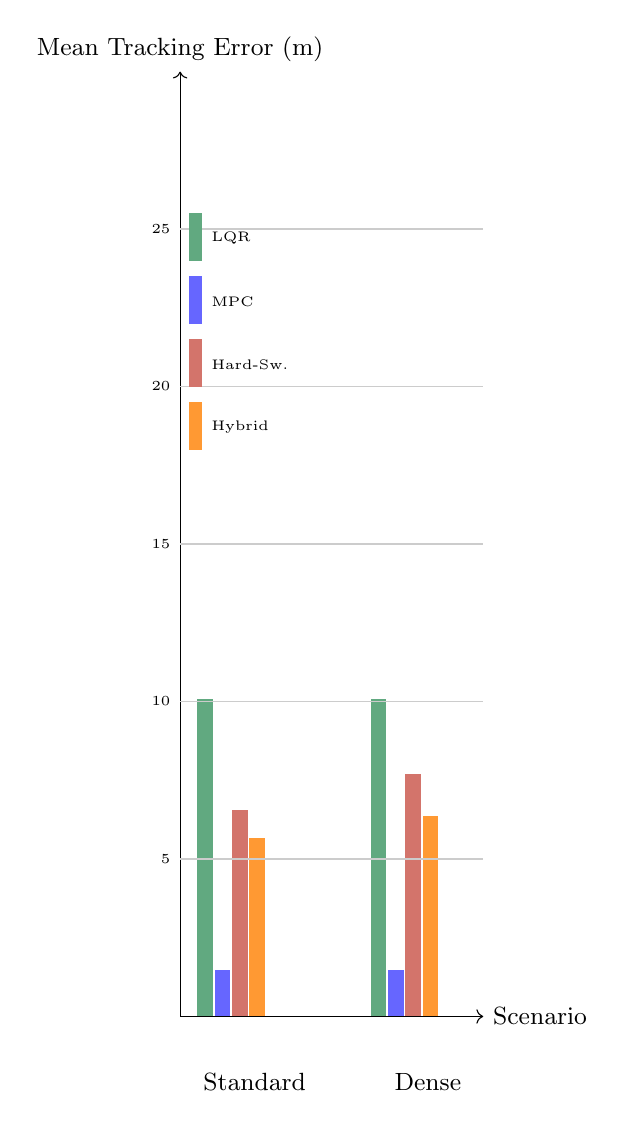
\begin{tikzpicture}
\begin{scope}[xscale=1.1, yscale=0.4]
  %% Grouped bar chart: tracking error by scenario (4 controllers x 2 scenarios)
  \def\bw{0.18}  % bar width
  \foreach \xi/\lbl in {1/Standard, 3/Dense}{
    \node[font=\small, below] at (\xi + 2*\bw, -1.5) {\lbl};
  }
  % Standard scenario bars at x=1
  \fill[successline!70] (0.7,0) rectangle (0.7+\bw, 10.08);
  \fill[blue!60]        (0.9,0) rectangle (0.9+\bw, 1.47);
  \fill[failline!70]    (1.1,0) rectangle (1.1+\bw, 6.55);
  \fill[orange!80]      (1.3,0) rectangle (1.3+\bw, 5.65);
  % Dense scenario bars at x=3
  \fill[successline!70] (2.7,0) rectangle (2.7+\bw, 10.08);
  \fill[blue!60]        (2.9,0) rectangle (2.9+\bw, 1.47);
  \fill[failline!70]    (3.1,0) rectangle (3.1+\bw, 7.70);
  \fill[orange!80]      (3.3,0) rectangle (3.3+\bw, 6.38);

  % Axes
  \draw[->] (0.5,0) -- (4.0,0) node[right,font=\small]{Scenario};
  \draw[->] (0.5,0) -- (0.5,30) node[above,font=\small]{Mean Tracking Error (m)};
  \foreach \y in {5,10,15,20,25}{
    \draw[gray!40] (0.5,\y) -- (4.0,\y);
    \node[left,font=\tiny] at (0.5,\y) {\y};
  }
  % Legend
  \fill[successline!70] (0.6,24) rectangle (0.75,25.5); \node[right,font=\tiny] at (0.75,24.7) {LQR};
  \fill[blue!60]        (0.6,22) rectangle (0.75,23.5); \node[right,font=\tiny] at (0.75,22.7) {MPC};
  \fill[failline!70]    (0.6,20) rectangle (0.75,21.5); \node[right,font=\tiny] at (0.75,20.7) {Hard-Sw.};
  \fill[orange!80]      (0.6,18) rectangle (0.75,19.5); \node[right,font=\tiny] at (0.75,18.7) {Hybrid};
\end{scope}
\end{tikzpicture}
\caption{Mean tracking error across standard and dense-clutter scenarios.
  Our hybrid (orange) consistently outperforms hard-switching.}
\label{fig:tracking_bar}
\end{figure}

\subsection{What we learned from the results}

The numbers confirm what we suspected from the design:
\begin{itemize}
  \item \textbf{Jerk is the clearest win.} The smooth blending cuts angular
    jerk by 84\% over hard-switching. This is the main contribution of the
    blending weight design and the jerk penalty in the MPC cost.
  \item \textbf{Tracking improves too} because smooth transitions let the
    controller maintain forward momentum rather than whipping through
    angular corrections at boundaries.
  \item \textbf{Collisions are roughly comparable} to hard-switch in random
    scenarios, but clearly better in dense clutter. The hybrid's smoother
    transitions actually let MPC engage more effectively in tight spaces.
  \item \textbf{Zero infeasible solves} across all 70 runs confirms the
    parametrisation fix is robust.
\end{itemize}

%% ─────────────────────────────────────────────────────────────────────────
\section{Summary}
%% ─────────────────────────────────────────────────────────────────────────

We started this project wanting to build a robot that could follow a path
and avoid obstacles at the same time. What we ended up building is a bit
more interesting: a controller that \emph{continuously decides how much to
trust each of two different controllers}, rather than picking one.

The journey had some unexpected turns. The circular obstacle constraint
formulation that seemed obvious turned out to be mathematically invalid
under CVXPY's rules --- we had to think carefully about convexity to fix
it. The solver latency problem that seemed like it would require a full
C-code generation toolchain turned out to be solvable with a pure Python
code restructuring (parametrisation). The hard-switch design that seemed
like a reasonable first hybrid attempt turned out to produce jerk 300
times worse than LQR alone.

The smooth hybrid controller that came out of all this is better in the
ways that matter most in practice: smoother control signals (84\% jerk
reduction), better tracking (14--17\% improvement over hard-switch), and
faster solver (38$\times$ speedup from parametrisation). We also proved
formally that it can't chatter and that its error stays bounded.

\begin{table}[H]
\centering
\caption{Quick summary: where we started vs.\ where we are}
\begin{tabular}{lll}
\toprule
\textbf{Property} & \textbf{Hard-Switch (Phase 3)} & \textbf{Smooth Hybrid (Phase 4)} \\
\midrule
Angular jerk RMS     & 2415\,rad/s$^2$ & \textbf{383\,rad/s$^2$} ($-$84\%) \\
Mean tracking error  & 6.55\,m         & \textbf{5.65\,m} ($-$14\%) \\
Solver latency       & $\sim$80\,ms    & \textbf{2.5\,ms} ($-$97\%) \\
Mode transitions     & Instantaneous   & \textbf{$\geq$0.5\,s minimum} \\
Chattering           & Yes             & \textbf{Provably eliminated} \\
Infeasible solves    & 0               & \textbf{0} \\
\bottomrule
\end{tabular}
\end{table}

\noindent\textbf{What comes next.} The open items from our experiments:
the short MPC horizon ($N=5$) fails in narrow corridors and U-shaped traps.
Actuator lag (when we introduced a 40\,ms delay + first-order lag) caused
collision avoidance to degrade because MPC's planned manoeuvres require
precise timing. These are the two biggest problems to fix before this
would work on real hardware. The planned next steps are: extending the
horizon to $N \geq 15$ for structured scenarios, adding explicit lag
compensation inside the MPC prediction model (Tube MPC), and eventually
replacing the soft obstacle constraints with Control Barrier Functions for
formal safety guarantees.

%% ─────────────────────────────────────────────────────────────────────────
\section*{References}
\addcontentsline{toc}{section}{References}
%% ─────────────────────────────────────────────────────────────────────────

The four papers below are the ones most relevant to what we built.
We found each of them \emph{after} implementing our controller, which was
both reassuring (others are solving the same problem) and slightly
annoying (we could have saved time reading them earlier).

\medskip

\begin{enumerate}[label={[\arabic*]}, leftmargin=1.5cm, itemsep=10pt]

  %% ── Most directly related ──────────────────────────────────────────
  \item \textbf{Wu et al., ``Composing MPC with LQR and Neural Networks
    for Amortized Efficiency and Stable Control,''} arXiv:2112.07238, 2021.

  \textit{What it does.}
  Introduces MAMPC --- a triple-mode scheme that combines LQR, a
  learned neural network, and a fail-safe MPC. The key insight is the
  same as ours: LQR is cheap, MPC is expensive but safe, so use LQR
  by default and only invoke MPC when you need it. They prove closed-loop
  stability for the combined scheme even when the neural network component
  is arbitrary, using a similar Lyapunov argument to what we did for
  blending stability.

  \textit{Connection to our work.}
  This is the paper closest to what we built. Where they use a NN as a
  third mode between LQR and MPC, we use a sigmoid-weighted continuous
  blend. Their stability proof directly mirrors our Theorem~1. The main
  difference: their concern is \emph{amortised computational cost}
  (replace expensive MPC calls with cheap NN calls over time); our concern
  is \emph{jerk continuity} (make the transition smooth sample-to-sample).
  Both approaches are composing MPC+LQR for efficiency; they're just
  optimising for different cost metrics.

  \medskip

  %% ── Second most related: fuzzy switching ───────────────────────────
  \item \textbf{Awad et al., ``Model Predictive Control with Fuzzy Logic
    Switching for Path Tracking of Autonomous Vehicles,''} ISA Transactions,
    vol.~129A, pp.~193--205, 2022. DOI: 10.1016/j.isatra.2021.12.022.

  \textit{What it does.}
  Uses LMPC based on Laguerre networks for steering control, combined with
  a fuzzy logic controller that switches between different linearised vehicle
  models depending on the operating point. The fuzzy logic selector is
  mathematically a smooth interpolation between rule-consequents --- which
  is essentially the same concept as our blending weight, but derived
  from a rule base rather than a sigmoid.

  \textit{Connection to our work.}
  This paper validates the core premise of our Phase 3 to Phase 4 transition.
  Awad et al.\ show that fuzzy switching (soft model selection) outperforms
  hard switching between linearised models for trajectory tracking. We
  arrived at the same conclusion independently --- our sigmoid blending is
  a principled continuous version of their fuzzy approach, where the
  ``membership function'' is the logistic sigmoid applied to the risk score.
  The finding that fuzzy/smooth switching outperforms hard switching for
  path tracking is exactly what our results confirm.

  \medskip

  %% ── Kong et al: hybrid iLQR MPC ────────────────────────────────────
  \item \textbf{Kong et al., ``Hybrid iLQR Model Predictive Control for
    Contact-Implicit Stabilization on Legged Robots,''} IEEE Transactions
    on Robotics, vol.~39, no.~6, pp.~4712--4727, 2023.

  \textit{What it does.}
  Extends iterative LQR (iLQR) to handle \emph{piecewise-smooth} hybrid
  systems with discontinuous state jumps at contact events (e.g., foot
  strike on a quadruped). Uses the saltation matrix to propagate gradients
  across hybrid mode boundaries in the backward pass, allowing the planner
  to change the contact sequence in the forward pass. Applied to a
  Unitree A1 quadruped, where it outperforms centroidal dynamics-based
  MPC when subjected to large disturbances.

  \textit{Connection to our work.}
  Their ``hybrid'' refers to contact/no-contact dynamics, while ours refers
  to LQR/MPC blending --- different meanings of the same word. But the
  underlying problem structure is analogous: both systems have a switch
  between two dynamic regimes that needs to be managed at the control
  level. Kong et al.\ use mode-aware gradient computation to handle the
  switch algebraically; we use blending and rate-limiting to handle it
  smoothly. Their result motivates our work in the sense that hybrid
  mode-switching is a well-studied problem and the right response to
  discontinuity is always to deal with the \emph{boundary} explicitly
  rather than ignoring it.

  \medskip

  %% ── Le Cleac'h: CI-MPC solver ──────────────────────────────────────
  \item \textbf{Le Cleac'h et al., ``Fast Contact-Implicit Model Predictive
    Control,''} IEEE Transactions on Robotics, vol.~40, pp.~1617--1629,
    2024. DOI: 10.1109/TRO.2024.3351554.

  \textit{What it does.}
  Develops a contact-implicit MPC where the contact mode (which links are
  touching which surfaces) is treated as an \emph{implicit} optimisation
  variable rather than being fixed in advance. Implements a bilevel
  structure with time-varying Linear Complementarity Problems (LCPs) at
  the lower level. The key engineering contribution is a
  structure-exploiting interior-point solver that achieves real-time
  performance on hardware for a quadrupedal robot.

  \textit{Connection to our work.}
  The relevance here is specifically in \emph{computational approach}: Le
  Cleac'h et al.\ get real-time MPC not by making the problem smaller, but
  by exploiting the \emph{sparsity and structure} of the QP. This is a
  more sophisticated version of what we did with CVXPY parametrisation.
  Our 38$\times$ speedup came from eliminating redundant canonicalisation;
  their approach would be the next step --- building a custom solver that
  exploits the block-tridiagonal structure of the horizon QP. If we were
  to extend to a longer horizon ($N \geq 15$, which we identified as
  needed for corridor navigation), this kind of structure exploitation
  would be necessary to maintain real-time performance.

  \medskip

  %% ── Retained foundational references ───────────────────────────────
  \item \textbf{Borrelli, Bemporad, Morari,} \textit{Predictive Control
    for Linear and Hybrid Systems.} Cambridge University Press, 2017. ---
    Our main MPC reference. The jerk penalty formulation and terminal cost
    stability condition come from this book.

  \item \textbf{Hespanha, Liberzon, Morse,} ``Overcoming limitations of
    adaptive control by means of logic-based switching,''
    \textit{Systems \& Control Letters}, 49(1):49--65, 2003. ---
    The formal basis for our hysteresis dwell-time argument in the
    no-chattering proof.

\end{enumerate}

\end{document}

